\section{Introduction}\label{intro}
Implementing an automated poker player is challenging since poker involves
elements of uncertainty, randomness, strategic interaction, and game-theoretic
reasoning. Heads-up poker is a form of Texas Hold'em poker that is played 
between two players. In this project, we aim to discuss implementing an 
automated heads-up poker player. Our approach to this problem is breaking
the problem into a sequence of simplified problems. 

The rest of this progress report is organize as follows: in \S 2 we describe the
rules of heads-up poker and the dynamics of the game. In \S 3 we will
demonstrate the hierarchy of simplified problems and their complexity.
\S 4 contains our main model for the project and \S 5 describes our implementation
so far. Finally, a discussion on our roadmap and future work is brought in \S6.

\section{Rules}
We are going to build our model based on \emph{Doyle's game} which was used 
in the 2007 Association for the Advancement of Artificial Intelligence (AAAI) 
Computer Poker Competition. The game is played between two players that we 
will call player A and player B. 

\BIT
\item \textbf{Blinds:} Every hand, both players start with 1000 chips. In odd hands (every other 
hand), player A is the \emph{small blind} and contributes 1 chip to the pot, while 
player B is the \emph{big blind} and contributes 2 chip to the pot. In even hands the 
role of two players is reversed. 
\item \textbf{Pre-flop:} Two players are dealt random cards (face down) which are called
\emph{hole cards}. Then the small blind can either \emph{fold} (\ie yield all the chips in
the pot to the other player), \emph{call} (contribute chips to the pot such that the number
of contributed chips from two players are equal), or \emph{raise} (contributing more chips
to the pot than the opponent). Notice that the famous \emph{all-in} action is a especial case
of raising. The betting process goes on until one player stops raising (and folds or simply calls).
\item \textbf{Flop:} Three community cards from the rest of the deck are shown. Starting from
the big blind, the betting process starts over similar to pre-flop. Unlike pre-flop where the
players are only using their hole cards to make actions, here the players are getting more
information about the community cards.
\item \textbf{Turn:} A fourth community card dealt face up. The betting process is similar to
flop.
\item \textbf{River:} A fifth (and last) community card is shown. A final round of bets takes place
similar to flop and turn.
\item \textbf{Show down:} In the event that none of the players fold until the end of river round,
two players make the best combination of five cards out of seven cards (two hole cards and 
five community cards). The player with a better combination wins the pot. In the case of
two equally ranked hands, the pot is split.
\EIT

\section{Literature review}
Poker is one of the most popular card games played around the world.
It has a rich story of study among game theorists, mathematicians, 
and economists. Recently, there has been lots  of research into 
developing strong programs for playing poker. In [1] authors introduced
the Bayesian Poker Program (BPP), which uses a Bayesian network to model 
poker hands and the opponent's playing behavior. In [2] an algorithm
to compute the approximate jam/fold equilibrium strategies in tournaments 
with three players has been developed. In a jam/fold strategy, all
players can only fold or go all in (jam). This strategy known to be 
the near-optimal in the two player tournaments. A heads-up no-limit Texas 
Hold'em poker player called Tartanian, has been introduced in [3]. Tartanian
uses a discretized betting model to reduce the size of the strategy space.
It also, benefits from a card abstraction model to decrease the problem size.
In [4] a poker program called Poki has been developed. Poki uses reinforcement 
learning techniques to explore and construct statistical models for each opponent,
 and exploit based on the observed patterns. 
 
\section{Implementation0}
In this project we will implement the limited Texas Hold'em heads-up poker. As we
described in section 2, every hand proceeds in four states \{{\tt pre-flop}, {\tt folp}, 
{\tt turn}, {\tt river}\}. In each state of a hand, there will be a bidding action 
between agents, then if they concur on the bidding value, the hand will
step into the next state. In the limited poker, the set of all valid actions 
for agents is \{{\tt fold}, {\tt check}, {\tt bet}\}. In our model, for each agent
we define two hidden random variables $F$, and $H$, which are not revealed to the
opponent. $F$, is a feature vector representing the agent's properties, i.e. her 
level of aggression. $F$ can be quite complicated, to incorporate the 
agent's way of playing in all levels. In our model we only consider one feature 
to represent how much aggressive/conservative the agent is. $H$ is a random
variable representing the agent's hole cards. Note that $H$ is unique for 
each hand of the game and $F$ is unique for each agent.
\\
\emph{How the agent plays poker?}\\
The agent will consider two hidden random variables $H$ and $F$ as described above 
for the opponent and tries to update her beliefs about them as she plays. Figure (1) shows the
PGM model for each state of a particular hand that the agent uses to update her 
bleifs. In this model, $B$ represents the dealt cards so far on the board, $S$ is the 
story of the hand so far (i.e. the actions in the previous states of the hand), and 
$A$ is the opponent's action. Note that $B$, $S$, and $A$ are all observed by the
agent, and she should use them to update her beliefs about hidden random variable
$H$.
 
\begin{figure}[h!]
  	\centering
 	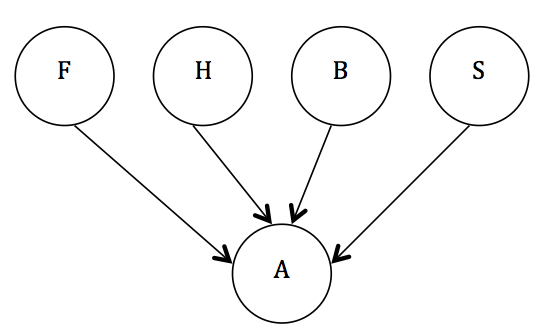
\includegraphics[scale = .55]{fig1}
\end{figure}

 
\section{Implementation}
We use Python for our implementation. We have a class {\tt pokerCards} that consists
two subclasses {\tt card} and {\tt deck}. Each {\tt card} has two parameters rank and suit.
Rank is a number in $\{2,3,\cdots,14\}$ (where 14 means Ace) and suit is a number in 
$\{1,2,3,4\}$. The {\tt deck} has methods like pop and shuffle.

We also have another class {\tt handEvaluator} that contains functions to evaluate poker hands.
In particular, the method we use is inspired by [1]. The idea here is to assign scores to sets of
five, six, or seven cards such that the hand with higher rank has a higher score and equally-ranked
hands have the exact score. Specifically, {\tt handEvaluator} function receives the hole cards and  
the board (with three to five cards) as its arguments and assigns a real number in $[0,1]$
to the union of hole cards and the board. If {\tt handEvaluator(h1,b) > handEvaluator(h2,b)},
it means that the rank of best five cards in {\tt h1$\cup$b} is higher than the best five cards
in {\tt h2$\cup$b}. Notice that this doesn't mean the {\tt h1} does not have any chance to win.
